\section{Proteínas}
\cite{tamar}
El término \textbf{proteína} se origina del griego \textit{proteios},
que significa ``primario'' o ``de primer orden''. El nombre fue
adoptado por Jöns Berzelius en 1838 para enfatizar la importancia de
esta clase de moléculas. Las proteínas juegan un rol crucial en el
mantenimiento de la vida (/sout{life-sustaining}). Las proteínas
proveen el soporte para la arquitectura de tejido musculoso,
ligamentos, tendones, huesos, piel, cabello, órganos y glándulas. Las
proteínas también proveen los servicios fundamentales de transporte y
almacenamiento como en el caso del oxígeno y hierro en células
musculares y \sout{de sangre}. Las proteínas también juegan un rol
crucial en muchos procesos regulatorios esenciales para la vida, como
reacciones de catálisis (e.g. digestión); funciones inmunológicas y
hormonales;  y la coordinación de actividades neuronales, crecimiento
de células y hueso, y diferenciación celular.

\begin{figure}[h]
  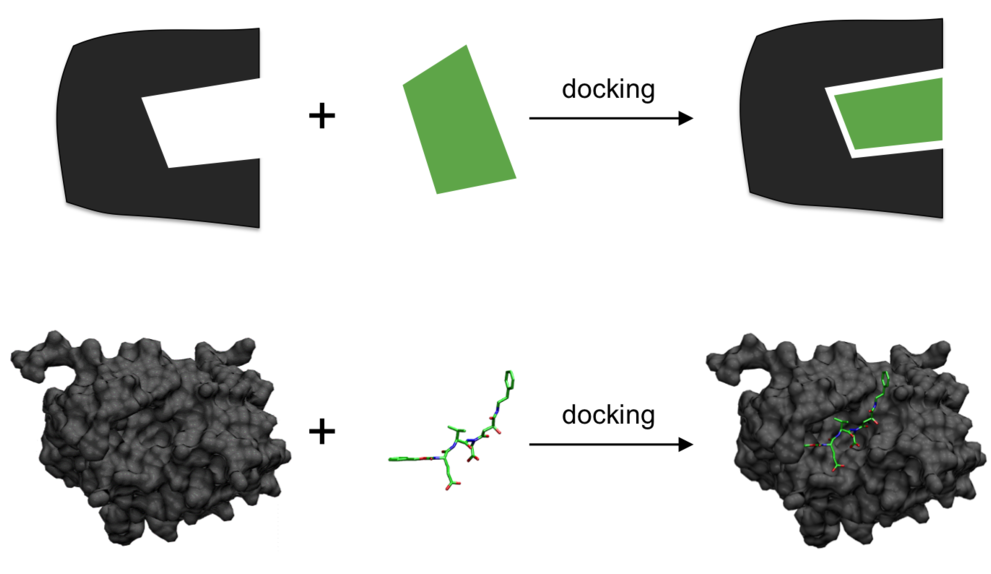
\includegraphics[scale=0.3]{docking}
  \centering
  \caption{Representación esquemática del \textit{docking}.
    (Tomado de \url{https://en.wikipedia.org/wiki/Docking_(molecular)})}
\end{figure}

\subsection{Acoplamiento molecular}
Basado en \cite{kukol}
El campo del \textbf{acoplamiento molecular} o \textbf{docking}
surge a lo largo de las últimas tres décadas gracias a la necesidad de la
biología molecular estructural y el descubrimiento de hinibidores basado
en estructuras. Ha podido evolucionar considerablemente gracias al
crecimiento dramático de disponibilidad y poder de las computadoras, y
al creciente acceso a bases de datos de proteínas y moléculas.

El objetivo de un programa de acoplamiento molecular automatizado es
comprender y predecir reconocimiento molecular, tanto
estructuralmente, encontrando posibles \textit{poses} de acoplamiento,
como energéticamente, prediciendo la afinidad del enlace. El
acoplamiento molecular usualmente se realiza entre una molécula
pequeña, llamada ligando, y una macromolécula objetivo, una proteína
en nuestro caso.

\begin{figure}[h]
  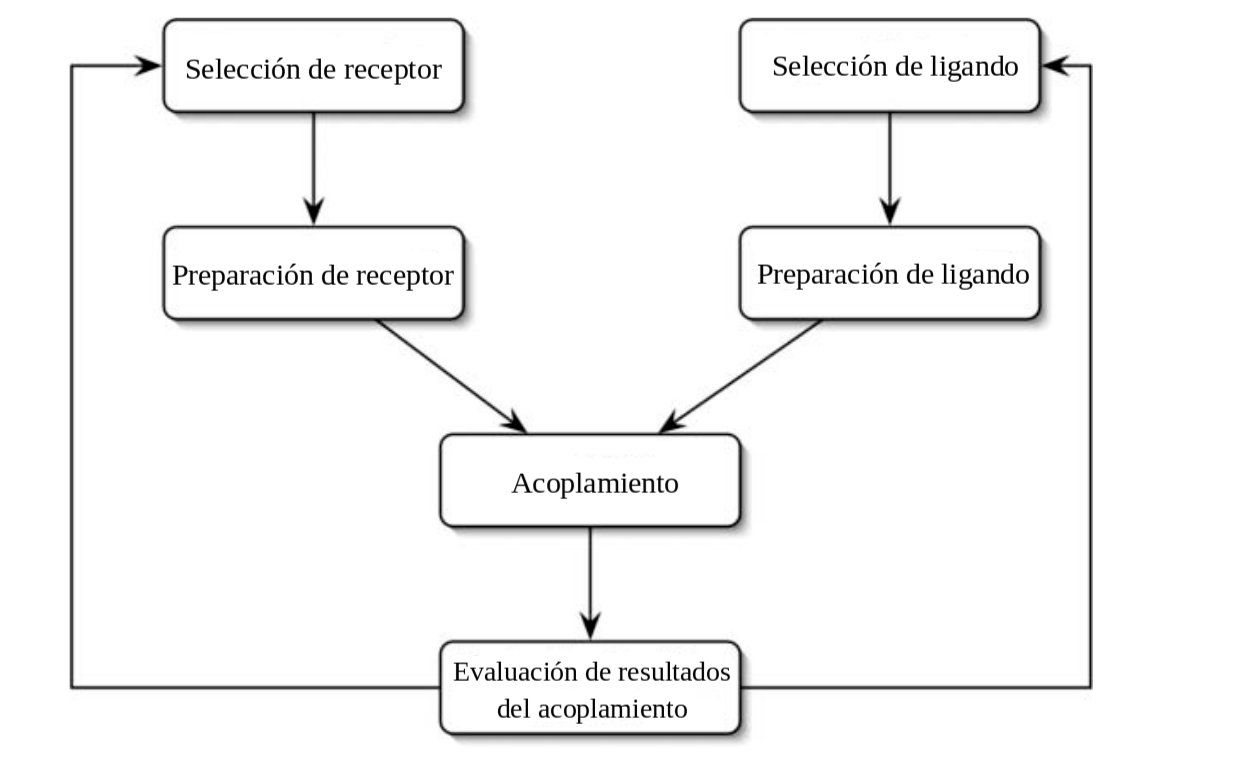
\includegraphics[scale=0.5]{docking_steps}
  \caption{Diagrama de flujo para un acoplamiento usual.
    (Tomado de \cite{kukol})}
  \label{fig:docking_flowchart}
\end{figure}
\ref{fig:docking_flowchart} muestra los pasos clave que son comunes en
todos los protocolos. El acoplamiento consiste en encontrar los
\sout{binding modes} más favorables de un ligando hacia una proteína
objetivo. El \sout{binding mode} de un ligando puede ser caracterizado
de forma única por sus variables de estado. Estas consisten en su
posición (traslaciones sobre los ejes $x, y, z$), orientación (ángulos
de Euler o cuaterniones) y, si el ligando es flexible, su conformación
(los ángulos de torción para cada enlace \sout{rotable}). Cada una de
las variables de estado describe un grado de libertad en un espacio de
búsqueda multidimensional.

\subsection{Función evaluadora}
Todos los métodos de acoplamiento requieren una función de evaluación
para calificar los \sout{binding modes} de los candidatos, y un método
de búsqueda para explorar las configuraciones de las variables de
estado. En general, el éxito de un acoplamiento se mide en términos de
la \textit{desviación media cuadrática} (RMSD) de las coordenadas
cartesianas de los átomos del ligando en las conformaciones del
acoplamiento, comparadas con las cristalográficas: un acoplamiento se
considera exitoso si el RMSD es menor a 2\AA.

\subsection{Archivos PDB}
El banco de datos de proteínas es un archivo de estructuras de macromoléculas
biológicas determinadas experimentalmente. El formato utilizado para almacenar
está información contiene elementos como coordenadas de átomos, nombres de
moléculas e información sobre estructuras primarias y secundarias. Es con este
formato con el que se trabajó durante el proyecto.
\footnote{\url{ftp://ftp.wwpdb.org/pub/pdb/doc/format_descriptions/Format_v33_Letter.pdf}}

\subsection{SMILES}
SMILES (Simple Molecular Input Line Entry System) es un sencillo lenguaje
químico que permite describir moléculas y reacciones utilizando únicamente
caracteres ASCII que representan símbolos de átomos y enlaces. Una cadena SMILES
contiene la misma información que una tabla de conexiones extendida, pero con
varias ventajas: es sumamente compacta y puede ser canonizada de tal manera
que puede ser usada como identificador universal para una estructura química
dada.\footnote{\url{http://www.daylight.com/smiles/}}
